\section{Background} \label{background}

A literature study has been conducted to situate the thesis topic. Multiple subjects lay at the base of the design described in section \ref{design}. Of these subjects, three are key which are explained first: electronic health record systems, telemonitoring and dashboard design. The process followed to create the final prototype is explained hereafter. Finally, topics that should be kept in mind when developing health software are briefly described, as they are not part of the scope of the prototype.

    \subsection{Electronic health record systems}

    Health information systems are becoming an important part of health care. They not only support patient care but also administrative and financial tools. At the heart of these systems lies the electronic health record. An electronic health record (EHR) is a repository of electronically maintained information about an individual's health status and health care, stored such that it can serve multiple legitimate uses and users of the record \cite{biomedical_informatics}. An electronic health record system (EHRS) provides tools to manage and interact with these records. These tools include providing reminders, data analysis, and decision support. It helps the clinician to organize, interpret and react to data.

    First, the advantages of EHRS over paper-based records are described to signify its importance. Secondly, the main components present in these systems are summarized. The functionality of an EHRS can be categorized into two types: a monolithic system tries to provide more general care, while smaller and more specialized systems cater to more specific types of care. The last section compares the two types and highlights the benefits and drawbacks of both.

        % signify importance
        \subsubsection{Moving away from paper} \label{2_ehrs_paper}

        For modern medicine, the traditional paper-based medical records are not suited in today's world filled with technology. The drawbacks of information on paper are obvious when compared to digitally stored information.

        \paragraph{Functionality} Digital records allow systems to aggregate, process and generate statistics of the data it contains. For example, heart rate graphs with typical statistics can be generated and when the users hover over a data point in the graph, the exact value is shown. Paper records containing tables or printed graphs that show the same data are limited in this regard.

        A paper-based medical dossier can store medical images, such as x-rays, but compared to a digital image, a lot of detail is lost. As such, other multimedia types cannot be stored on paper. With an EHRS, these file types can be attached with ease, provided the system supports them. Paired with the tools of the health system, a lot more functionality can be achieved.

        In terms of data input, an EHRS can detect and prevent false data input. The system can make sure all necessary data fields filled in and in the correct format. This results in more complete and accurate data gathering with fewer errors.

        \paragraph{Information quality} A summarizing paper noted that the use of EHRS leads to more complete, accurate, comprehensive and reliable data compared to paper-based records \cite{ehrs_summary}. As mentioned in the previous paragraph, a digital system can impose rules on data fields to avoid missing or entering the wrong data. In terms of comprehensibility, poor handwriting leads to wrong or loss of information, which is avoided on digital systems.

        \paragraph{Accessibility} Paper records are difficult to access because most of the time only one copy exists. Transferring these records to other branches or institutions, therefore, is difficult: the record has to be found in the often large medical dossier, has to be copied and then manually sent. Also, misfiling, flooding or fires can lead to irrecoverable loss of the data. Digital records avoid the last issue, but there can still be difficulties regarding data transfer as most institutions have their own database structures.

        The process of moving data on paper to a digital format requires a lot of manual work. While some aspects can be automated, such as scanning and processing the paper forms with software, verification is still necessary. All the data fields from the documents need to find a place in the EHR, which frequently is not possible. Also, what do we do with unreadable data due to poor handwriting? What happens with duplicate forms with slightly different values? Because of these reasons, adopting an EHRS is a significant undertaking for an institution. As such, the benefits are not immediately apparent.

        Because digital storage increases accessibility significantly, security measurements have to be taken. If not, data can be stolen, deleted or even altered. This also adds to the complexity of developing EHRS.

        % wip
        \paragraph{Efficiency} An important task of an EHRS is to facilitate effective care. An early study saw a 6\% increase in productivity when EHRS were deployed in health care institutions \cite{ehrs_efficiency}. However, other factors are at play, such as the adoption rate. The transition from paper-based documenting to digital is accompanied by a learning curve, which can be steep. After the switch, the productivity will be lower at the start and as the users become more experienced with the software, it will increase.

        \subsubsection{Components of an EHRS}

        As mentioned before, EHRS do not simply store patient records. They consist of many components which ultimately define how well they perform in health care. Literature gives us multiple definitions of which components are essential. However, we summarize them in the following five \cite{biomedical_informatics}:

        \paragraph{Integrated view of patient data} An EHR must allow storage of a wide range of data types. This can be text, numbers, images, video, and others. Some data can still be on paper due to lacking support of the EHRS, as mentioned in section \ref{2_ehrs_paper}. To display more complex data types, such as x-ray images, standards are used. A brief overview of such standards can be found in section \ref{2_standards}.

        \paragraph{Clinician order entry} Order entry is the point at which the clinician has to make decisions or take action. An order entry system can assist the clinician by providing decision support. It also reduces errors and costs compared to paper order entry.

        \paragraph{Clinical decision support} A decision support system embed into an EHRS can aid the clinician by suggesting actions to take, when certain situations occur. If for example, a patient is due for a vaccination, the system can notify the clinician by presenting a constructed order which needs to be confirmed or denied. The system can do this for a bulk of patients, so manual checkups are not required, thus saving time.

        \paragraph{Access to knowledge resources} When clinicians are writing notes or orders for a patient, clinical questions can arise. Instead of asking colleagues, the EHRS can pull literature to address the question. Due to the internet, a very large source of information is readily available.

        \paragraph{Integrated communication and reporting support} Communication is an important part of health care. Often clinicians of multiple institutions provide care for a particular patient. The effectiveness of patient care, therefore, is directly affected by communication which is why EHRS should provide tools to assist the clinicians. Most institutions are bounded by their own EHRS, which requires them to ask the other institutions for necessary data. A solution to this problem is Health Information Exchange, which allows institutions to reach data beyond their own EHRS.\\
        
        \noindent Throughout the years, many EHRS have been developed which may or may not integrate all of the above components. Should an essential component be missing, an institution may add another system. Although this has its benefits and drawbacks.

        \subsubsection{Monolithic vs. multiple EHRS} \label{ehrs_comparison}

        Health care institutions can opt for a monolithic EHRS or combine multiple EHRS to achieve all required functionality. To both there advantages and drawbacks \cite{multiple_ehrs}. Elements influencing this choice include IT infrastructure, safety risks, the volume of care and frequency with which patients move facilities. However, it's possible that a single EHRS does not satisfy the requirements of an institution. A reason for this is that certain branches require specially tailored software for their clinical practice, which a general EHRS lacks. 

        Functionality wise, a monolithic EHRS tends to appeal to more general types of care, whereas it lacks in very specific ones. Also, vendors that offer these all-in-one solutions have less experience with these specialties which reduces the chance it will be added to the system. Vendors of specific EHRS do have this expertise and can tailor the system to the needs of the customer. In this case, combining a system that supports general care with special care systems will seem like the best choice. However, other considerations have to be made.

        The advantage of a monolithic system is that the data it uses is centralized. This ensures that all data can be accessed anywhere in the system and that it can be easier maintained. When multiple systems are in place, data has to be exchanged and can lead to difficulties finding certain pieces of information. The exchange of data is difficult, as each system probably has its own data structures. A potential solution is to create a new EHRS, solely for the purpose of data collection and transformation with which all systems interface with. This leads to another system, requiring additional development and maintenance time.
    
    \subsection{Telemonitoring} \label{2_telemonitoring}
    % between consultations
    % in relation to EHRS
    % transfers burden partly to patient
    Monitoring patients at a distance with the use of information technology is called telemonitoring \cite{systematic_review}. The patient uses special monitoring devices to gather data which is sent to the health care provider. While many health conditions can be monitored, telemonitoring is most prevalent in chronic diseases due to their long-lasting nature and necessity to self-manage. Two of these diseases, heart disease and cancer, accounted for 46\% of all deaths in the United States \cite{national2016health}. Also, 86\% of all health care spending is for patients with one or more chronic conditions \cite{gerteis2014multiple}. A study has shown that not only the complications of chronic conditions and costs can be reduced by the use of telemonitoring: care can be provided without the use of hospital beds and the time spent managing the disease is lower \cite{telemonitoring_current_state}.

    First, an overview of how telemonitoring has been applied to chronic conditions treatment is given. Second, the difficulties surrounding telemonitoring are mentioned.

        % 4 WHO categories -> no cancer
        \subsubsection{Chronic conditions}

        A chronic condition can be defined as a long-lasting human health condition. If the length of the condition is at least three months, the term chronic is used. The WHO defines four major categories of chronic diseases: cardiovascular diseases, cancer, diabetes and chronic respiratory diseases \cite{world2017noncommunicable}. Due to a lack of literature on telemonitoring in relation to cancer, only the other categories will be discussed. The respiratory disease category focusses on chronic obstructive pulmonary disease.

        \paragraph{Cardiovascular diseases} A study recruited 390 patients to test the effect of telemonitoring to reduce hospital days and total costs \cite{tompkins2010randomized}. 193 individuals were in the intervention group and were to take daily measurements using specialized hardware. The hardware was capable of recording the weight, blood pressure, heart rate and blood oxygen levels. If the patient had diabetes, an additional blood glucose meter was provided. Patients were also required to fill in a predetermined set of questions every week. On the clinician's end, nurses were shown a summarizing table indicating if the sent results were good, bad or missing. Based on these results, the nurses would decide to contact the patient if extra care was needed.

        The study concluded that telemonitoring appears to facilitate more efficient outpatient care and potentially reduce costs. The total numbers of hospital days for the patients in the intervention group showed a tendency to be lower and fewer emergency department visits. However, there were more urgent care and primary care visits.

        Another research paper reviewed 30 studies and noted that most patients had a positive experience and little difficulty with telemonitoring technology \cite{inglis2010structured}. In total there were more than 9500 patients in the studies. The summary concluded that there were fewer deaths, fewer hospital admissions and improved quality of life. There were also hints of reduced cost, but some studies did not report on this topic. None of the studies reported on the optimal duration of for telemonitoring.
        
        The effect of telemonitoring treatment on cardiovascular patients is still unclear. A paper criticized the aforementioned one, stating that the conclusions made were only valid for small studies. For large trail studies, there was no significant effect \cite{chaudhry2010telemonitoring}.

        \paragraph{Diabetes} Due to the majority of research reporting on telemonitoring for diabetes type 2, type 1 will not be considered in the scope of this thesis. Due to it being a long-term disorder, combining the management of diabetes with telemonitoring is well documented in literature.

        One study required 32 patients to take blood glucose measurements for nine months using a Bluetooth capable glucose meter. The measurements would be sent to a mobile phone which in turn would forward them to a hospital server. Based on the measurements clinicians would review them and send recommendations to the patient and their general practitioner. The results showed a decrease in HbA\textsubscript{1C} from 8.40\% to 7.76\%. Due to the low amount of patients, the final conclusion said that the benefit of telemonitoring would likely be small \cite{istepanian2009evaluation}.

        Diabetes also has an effect on blood pressure, as approximately 50 to 80\% of diabetes type 2 patients suffer from hypertension which can lead to cardiovascular disease. A target blood pressure for diabetes patients would be 130/80 \cite{landsberg2004diabetes}. One study kept this goal in mind and developed a home telemonitoring program \cite{logan2012effect}. It is labeled as `home' due to the fact that a smartphone generates self-care messages for the patient, based on multiple previous readings. The results, however, would still be sent towards the clinician. Careful reviewing and responding to the patient would not be necessary, ultimately saving the clinician time. There were 55 patients in the telemonitoring group and as well in the control group. Both groups were required to measure their blood pressure using a device, but only the telemonitoring group had the device connected to a smartphone, generating the self-care messages. The results showed that the blood pressure only decreased significantly in the telemonitoring group. Also, the percentage that reached the 130/80 target blood pressure was 51\% for the telemonitoring group and only 31\% for the control group. Lastly, the self-caring nature of the program resulted in worsened depression compared to the control group.

        Weight loss also influences blood sugar. The Active Body Control Program reported the effects of telemonitoring in combination with a dietary program \cite{luley2011weight}. The subjects were obese with diabetes type 2. They were a weighing scale, an accelerometer and a device which would gather the measurements and send them to the hospital server. After six months significant improvements in blood sugar and weight loss were observed. No relevant changes were observed in the control group.

        Lastly, medication management is also linked to telemonitoring and diabetes. A study asked 64 patients (the telemonitoring group) to measure their blood glucose, blood pressure and weight on a daily basis \cite{stone2009active}. A nurse would receive these measurements and adjust the medication intake five times a week. The control group consisted of 73 patients who took measurements of the same parameters, but they only received a phone call once a month to have their medication schedule adjusted. The results noted a significant decrease in HbA\textsubscript{1C} for the telemonitoring group after three and six months, compared to the control group.

        \paragraph{Chronic obstructive pulmonary disease} resp

        \noindent Test


        % data accuracy, adherence, integration EHRS, training of users...
        \subsubsection{Difficulties}

    \subsection{Dashboards} \label{2_dashboards}

    The primary goal of a dashboard is clear communication, which is achieved with an effective design. A formal definition is as follows: ``A dashboard is a visual display of the most important information need to achieve one or more objectives; consolidated and arranged on a single screen so information can be monitored at a glance.'' \cite{dashboard}. This definition mentions four key characteristics:

    \paragraph{Dashboards are visual displays.} It is important that data is represented visually. Displaying charts and other graphics allows more efficient communication compared to textual information. For example, trends and outliers are easier to spot in a line chart compared to a table with the same values.

    \paragraph{Dashboards display information needed to achieve specific objectives.} The data that is shown, must be of use for the job that needs to be done. It is possible that the data needs to be gathered from multiple sources and tailored to the specific context so an efficient visualization can be created.

    \paragraph{A dashboard fits on a single computer screen.} In order to see all information at a glance, scrolling must be prevented. If multiple screens are present, then it is no longer a single dashboard. This leads to another question: what type of display is the information shown on? Due to the wide variety of screen sizes and aspect ratios, a responsive dashboard would be most beneficial.

    \paragraph{Dashboards are used to monitor information at a glance.} Important data should be immediately noticed, whereas very specific details should be hidden. This means data must be summarized or aggregated in order to be effectively shown. However, if the user wishes to view the detailed data, the dashboard should provide a way to do so.\\

    \noindent To create an effective dashboard, the user-base must be known and well understood. 
    
    Another important factor is the user type. Some users can understand one visualization better compared to the other. In order to create an effective dashboard, the focus should be put on the user \cite{brath2004dashboard}.
    
    
    Many EHRS fail to provide a meaningful dashboard. We only look at open-source systems as most health software is purchased and licensed.

    % wide range of dashboard types: monitoring stocks, network management...
    % examples of EHRS -> visually difficult
    % what makes a dashboard effective

    \subsection{MuiCSer} \label{2_muicser}
    % description of process
    This section describes the MuiCSer framework, made for user-centered software engineering processes in a multidisciplinary context \cite{muicser}, which will be used to create the prototype. This framework focuses on optimizing the user experience during the entire software engineering cycle to ensure that the end-user's needs are fulfilled. By combining user-centered design and software engineering principles the user experience of the final product can be improved substantially of the final product.

        \subsubsection{Process}
        
        \begin{figure}[!t]
            \centering
            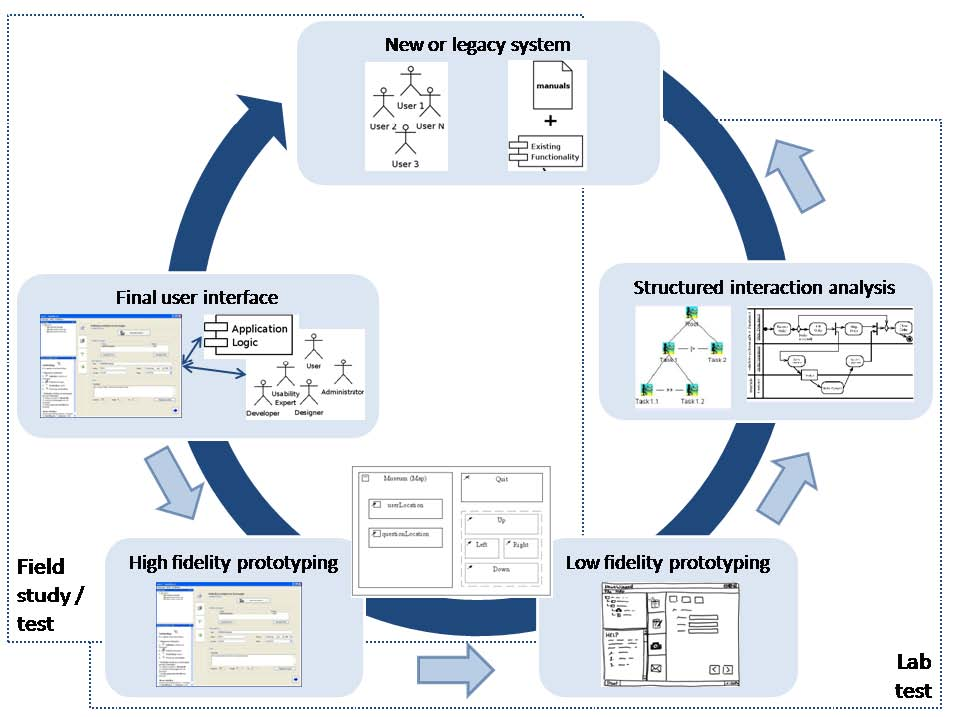
\includegraphics[width=0.8\textwidth]{chapters/2_background/muicser}
            \caption{MuiCSer process}\label{fig:muicser}
        \end{figure}

        The MuiCSer process is summarized in figure \ref{fig:muicser}. After each phase, the result is evaluated, verified and validated to ensure that the required functionality is present. The received feedback can, in turn, be used to reiterate over the previous phase. On the figure, this is denoted with the light arrows, while the dark one represents the overall process direction.

        \paragraph{New or legacy system} At the start of the process an existing system in need of improvement is either evaluated or a new one has to be designed. This requires an analysis of the tasks and needs of the user, as well as the objects and resources required to perform these tasks. Personas and scenarios are the resulting artifacts of this phase. First, personas describe the personalities of the potential end users including hobbies, skills and the environment they surround themselves in \cite{persona_scenario}. Its goal is to uncover behavior patterns which can be of use when designing a user interface. Second, a scenario is a story describing the use of a fictitious system from the persona's point of view \cite{persona_scenario}. It tries to sketch the usage of the system for which a design must be made.

        \paragraph{Structured interaction analysis} During this phase, the results of the analysis are used to create task models. These models specify concrete tasks and goals which can be dissected into specific actions or steps the user has to take. These artifacts lay the foundation for designing a user interface which supports these tasks and goals.

        \paragraph{Low fidelity prototyping} When the actions have been specified using the task models, low fidelity prototypes can be designed. Paper sketches and mockups are such examples and are ideal for visualizing the layout of the software its user interface. Without spending too much time and resources, presenting such prototypes can yield valuable feedback from the end-user or customer. However, there is no interaction present. Typically multiple versions of these prototypes will be created until the customer is satisfied after which high fidelity prototypes can be developed.

        \paragraph{High fidelity prototyping} Creating high fidelity prototypes requires a lot more effort compared to low fidelity prototypes, as they offer functionality closely resembling the final product. However, the feedback will be much more valuable as not only design, but also functionality is tested.

        \paragraph{Final user interface} When the latest iteration of the high fidelity prototype satisfies all user requirements, the final user interface can be created. It would be beneficial to reuse the code from the prototype in order to save time and resources. As a final step, the task models are checked against the interface to check if all required functionality is present.\\


    \subsection{Customization}
    % effect on user satisfaction

    \subsection{Standards} \label{2_standards}

    \subsection{Privacy}
    % not focus, brief description of issues
    Although not being a main focus, it is important to highlight the privacy concerns regarding health information data.

    

        

        


